\documentclass{article}
\usepackage[a4paper, left=15mm, top=20mm, right=15mm,bottom=20mm]{geometry}
\usepackage{amsmath, amssymb, amsfonts}
\usepackage{fancyhdr}
\usepackage{graphicx}
\graphicspath{ {./images/} }
\usepackage{float}
\usepackage{hyperref}
\usepackage{lscape}
\usepackage{multirow}

\pagestyle{fancy}
\fancyhf{}
\lhead{ACC1701X}
\rhead{claudeonrs}
\rfoot{\thepage}
\usepackage{amsmath, amssymb, amsfonts, listings}
\usepackage{xcolor}
\usepackage{enumitem}
\setlist[itemize]{noitemsep, topsep=0pt}
\setlist[enumerate]{noitemsep, topsep=0pt}
\setlist[description]{noitemsep, topsep=0pt}


%New colors defined below
\definecolor{codegreen}{rgb}{0,0.6,0.4}
\definecolor{codegray}{rgb}{0.5,0.5,0.5}
\definecolor{codepurple}{rgb}{0.58,0,0.82}
\definecolor{backcolour}{rgb}{0.95,0.95,0.92}
\definecolor{commentgreen}{rgb}{0.4,0.8,0.6}
%Code listing style named "mystyle"
\lstdefinestyle{mystyle}{
  backgroundcolor=\color{backcolour},
  commentstyle=\color{red},
  keywordstyle=\color{blue},
  numberstyle=\tiny\color{codegray},
  stringstyle=\color{codegreen},
  basicstyle=\ttfamily,
  breakatwhitespace=false,
  breaklines=true,
  captionpos=b,
  keepspaces=true,
  numbers=left,
  numbersep=5pt,
  showspaces=false,
  showstringspaces=false,
  showtabs=false,
  tabsize=2
}

%"mystyle" code listing set
\lstset{style=mystyle}

\title{No Title}
\author{Claudeon R Susanto}
\date{}
\usepackage[T1]{fontenc}
\usepackage[utf8]{inputenc}
\usepackage[english]{babel}
\usepackage{lmodern}

\renewcommand{\familydefault}{\sfdefault}   % Supprime le serif (dyslexie)
\usepackage[font=sf, labelfont={sf}]{caption}
\usepackage{multicol}
\usepackage{makecell}
\renewcommand\theadalign{bc}
\renewcommand\theadfont{\bfseries}
\renewcommand\theadgape{\Gape[4pt]}
\renewcommand\cellgape{\Gape[4pt]}



% own commands
\newcommand{\eg}[0]{\textit{e.g. }}
\newcommand{\ie}[0]{\textit{i.e. }}
\newcommand{\impt}[0]{\textcolor{red}{\textbf{[IMPT] }}}


\renewcommand\thesubsection{\thesection.\arabic{subsection}}
\setlength{\columnseprule}{1pt}
\begin{document}
%\maketitle
\fontfamily{lmss}\selectfont
\begin{multicols}{2}
\section{Accounting in Business}
\begin{description}
	\item[in the aggregate] accumulate transactions of the same type over a certain period and report the data as one amount in the company's financial statements
	\item[accounting] the entire process of identifying, recording, and communicating economic events (bookkeeping is part of recording only)\\
\end{description}
\textbf{Who uses accounting data?}
\begin{itemize}[topsep=0pt]
	\item \textbf{Internal users}\\
	\underline{Managerial accounting} provides internal reports to help users make decisions about their companies
	\begin{itemize}
		\item Management
		\item Employees
	\end{itemize}
	\item \textbf{External users} (investors and creditors, etc.)\\
	\underline{Financial accounting} provides economic and financial information for investors, creditors, and other external users
	\begin{itemize}
		\item Lenders
		\item Investors
		\item Competitors
		\item Government agencies\\
		IRS:
		SEC:
		\item The press
	\end{itemize}
\end{itemize}
\textbf{Measurement principles} (used by IFRS)
\begin{itemize}
	\item \impt Follow trade-offs between \textbf{relevance} (makes a difference in decision making) and \textbf{faithful representation} (factual and accurate)
	\item \impt Enhancing qualitative characteristics (\textbf{Comparability, Verifiability, Timeliness, Understandability})
	\item \textbf{Historical cost} principle: record assets at their initial cost when it was purchased
	\item \textbf{Fair value} principle: assets and liabilities should be reported at fair value (\underline{price received to sell an asset or settle a liability})
	\begin{itemize}
		\item Only used when asses are actively traded, otherwise rarely used
		\item Also used when market value info is available for certain assets\\
	\end{itemize}
\end{itemize}
\textbf{Accounting assumptions}
\begin{itemize}
	\item \textbf{Monetary unit} assumption: include only data that can be expressed in money terms
	\item \textbf{Economic entity} assumption: activities of the entity are separate and distinct from the activities of its owner and all other economic entities
	\begin{itemize}
		\item Proprietorship
		\begin{itemize}
			\item owned by \textbf{one} person
			\item the owner receives any profits and suffers any losses
			\item the owner has \textbf{unlimited liability} (liable for all debts of business)
			\item \textbf{no legal distinction} between the business as an economic unit and the owner
			\item Accounting records of the business activities are kept \textbf{separate} from owner's personal records
		\end{itemize}
		\item Partnership
		\begin{itemize}
			\item owned by \textbf{two or more} persons associated as partners
			\item each owner has \textbf{unlimited personal liability}
			\item for accounting purposes, partnership transactions are kept \textbf{separate} from personal activities
		\end{itemize}
		\item Corporation
		\begin{itemize}
			\item \textbf{separate legal identity} under corporation law
			\item ownership is divided into \textbf{transferable shares}: shareholders may transfer part or all of their ownership shares to other investors at any time
			\item holders of shares enjoy \textbf{limited liability}
			\item \textbf{Unlimited life}; ownership can be transferred without dissolving the corporation
			\item \textbf{Double taxation}: company's income is taxed, and then dividends to stockholders are taxed again :(
			\item Need government regulation
		\end{itemize}
	\end{itemize}
\end{itemize}

\subsection{The Basic Accounting Equation}
$$\text{Assets} = \text{Liabilities} + \text{Equity}$$
\textbf{Assets}:  A resource controlled by the entity in the \textit{present} due to \textit{past} event that will give rise to \textit{future} benefits
	\begin{itemize}
		\item \underline{Cash}
		\item \underline{Accounts Receivable}
		\item \underline{Supplies}
		\item \underline{Equipment}
	\end{itemize}
\textbf{Liabilities}: A \textit{present} obligation arising from \textit{past} event that is expected to lead to a \textit{future} outflow of resources upon settlement
	 \begin{itemize}
	 	\item \underline{accounts payable}: purchase commodities/equipment on credit from suppliers
	 	\item \underline{note payable}: money borrowed
	 	\item \underline{salaries/wages payable}
	 	\item \underline{sales and real estate taxes payable}
	 	\item \impt Example: claim from an employee due to workplace accident which is highly likely to be settled in the future
	 \end{itemize}
\textbf{Equity}: the ownership claim on a company (residual equity after creditors' claims are satisfied)
	 \begin{itemize}
	 	\item \textbf{Share capital-ordinary}: paid in by shareholders in exchange for the ordinary shares they purchase
	 	\item \textbf{Retained earnings}
	 	\begin{itemize}
	 		\item \underline{Revenues}
	 		\item \underline{Expenses}
	 		\item \underline{Dividends}: increase in net assets, available to distribute to shareholders
	 	\end{itemize}
	 \end{itemize}

\subsection{Financial Statements}
\begin{enumerate}
	\item \textbf{Income statement (IS)} presents the revenues and expenses and resulting net  income or net loss for a specifi c period of time.
	\item \textbf{Retained earnings statement} summarizes the changes in retained earnings for a specific period of time.
	\item \textbf{Statement of financial position (SFP)} (sometimes referred to as a balance sheet) reports the assets, liabilities, and equity of a company at a specific date.
	\begin{itemize}
		\item Current and noncurrent assets/liabilities (can be turned into cash/settled within 1 year?)
		\item Preferably sorted from higher liquidity to lower
		\item \impt Assets recorded at \textbf{cost/book value}, not market value
		\item \impt Revenue vs Loss/Gain
		\item \impt Notes Payable vs Accounts Payable \\
		Notes: usually cash\\
		Accounts: usually owed to suppliers
	\end{itemize}
	\item \textbf{Statement of cash flows (SCF)} summarizes information about the cash inflows (receipts) and outflows (payments) for a specific period of time.
	$$\Delta Cash = CFO + CFI + CFF$$
	\item \textbf{Statement of comprehensive income (SCI)} presents other comprehensive income items that are not included in the determination of net income
\end{enumerate}

\section{The Mechanics of Accounting}
\begin{itemize}
	\item \impt \textbf{Prepaid rent} is an \textbf{asset}!\\
	The benefits are not going to happen now; but will happen in the future
	\item \impt \textbf{Unearned revenue} is a \textbf{liability}\\
	Has to be settled in the future
\end{itemize}
\end{multicols}
\begin{figure}[H]
	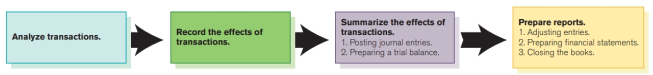
\includegraphics[width=\linewidth]{image/acc_cycle.png}
\end{figure}
%

\begin{multicols}{2}
	\begin{table}[H]
		\resizebox{\columnwidth}{!}{
			\begin{tabular}{c|c|c|c|ccc}
				& \multirow{2}{*}{Assets}  & \multirow{4}{*}{=} & \multirow{2}{*}{Liabilities} & \multicolumn{3}{c}{Equity}                             \\ \cline{5-7}
				&                &              &                 & \multicolumn{1}{c|}{Revenues} & \multicolumn{1}{c|}{Expenses} & Dividends \\ \cline{1-2} \cline{4-7}
				$\uparrow$& Dr.                  &                   &   Cr.                & Cr.                      &  Dr.                     & Dr. \\ \cline{1-2} \cline{4-7}
				$\downarrow$ &  Cr.                 &               &             Dr.      &   Dr.            &    Cr.                   & Cr.
			\end{tabular}
		}
	\end{table}
\section{Adjusting Accounts}
\textbf{Accrual Accounting} can capture the value of the firm much better due to timeliness\\
Adjusting entries made at the end of a period do not involve cash\\
Each adjusting entry involves a balance sheet account and an account on the IS/SCI;
\begin{itemize}
	\item \textbf{Unrecorded Receivables}: Amount that has not been paid but the work has been done/should be recognized (\eg billing every 3 months)
	\item \textbf{Unrecorded Liabilities}: Expenses being incurred prior to being paid or recorded (\eg interest payable, wages payable) in other words parts of expense is actually incurred due to the use of resources but it has not been paid
	\item \textbf{Prepaid Assets}: Payments that a company makes in advance for items charged to expense (\eg insurance premium payment) and the asset slowly loses its value
	\item \textbf{Unearned Revenues}: Amounts received before the actual recognition of revenues, and work is slowly being done over time which decreases liability and increases revenue
\end{itemize}
% Please add the following required packages to your document preamble:
% \usepackage{multirow}
\textbf{Accumulated Depreciation}: is a \textit{Contra-asset} with normal balance of credit
\begin{itemize}
	\item Note that for depreciation of PPE, PPE balance is not directly credited but instead Accumulated depreciation is credited (Less)
\end{itemize}
\textbf{Allowance for bad debt}: contra-asset for accounts receivable
\begin{table}[H]
	\resizebox{\columnwidth}{!}{
		\begin{tabular}{c|c|c|c|ccc}
			\multirow{2}{*}{} & \multirow{2}{*}{Assets} & \multirow{6}{*}{=} & \multirow{2}{*}{Liabilities} & \multicolumn{3}{c}{Equity}                             \\ \cline{5-7}
			&                   &                   &                   & \multicolumn{1}{c|}{Rev.} & \multicolumn{1}{c|}{Exp.} & Div.  \\ \cline{1-2} \cline{4-7}
			\makecell{Unrecorded \\Receivables}&  Dr.&  &  & Cr. &  &  \\ \cline{1-2} \cline{4-7}
			\makecell{Unrecorded \\Liabilities}&  &  & Cr. &  & Dr. &  \\ \cline{1-2} \cline{4-7}
			\makecell{Prepaid\\Expenses}&  Cr.&  &  &  & Dr. &  \\ \cline{1-2} \cline{4-7}
			\makecell{Unearned\\Revenues}&  &  & Dr.  & Cr. &  &
		\end{tabular}
	}
\end{table}

\textbf{Steps to preparing Financial Statements}
\begin{itemize}
	\item Adjust journal entries
	\item Adjust trial balance (book not closed yet)
	\item Prepare financial statements
	\begin{enumerate}
		\item IS $\rightarrow$ to calculate NI
		\item SCE $\rightarrow$ to calculate $\Delta$RE
		$$\text{RE}_1 + \text{NI} - \text{Dividends} = \text{RE}_2$$
		\item SFP (Classified)
	\end{enumerate}
    \item Close book
    \begin{itemize}
    	\item Transfer nominal accounts to RE
    \end{itemize}
    \item Post-closing trial balance
\end{itemize}

\section{Problems in Financial Statements}
\begin{enumerate}
	\item Errors (unintentional mistakes)\\
	not entering/forgot to enter, entering wrong info/amount, entering wrong accounts
	\item Disagreements on judgment\\
	Different parties have different judgments/estimates abt revenue accounts
	\item Frauds $\Rightarrow$ intentional in order to manipulate FS!
	\begin{itemize}
		\item \textbf{Corruption}: misusing one's position for personal gains
		\item \textbf{Asset Misappropriation}: Theft/embezzlement of company resources
		\item \textbf{Financial Statements Fraud}: misreporting amounts to portray more favourable results
	\end{itemize}
\end{enumerate}

\subsection{Fraud}
\textbf{The Fraud Triangle} (Why people commit fraud)
\begin{enumerate}
	\item Pressure\\
	pressure to meet financial/personal goals/attract investors
	\item Opportunity\\
	Weak internal control/adequate means to commit fraud
	\item Rationalization\\
	Justify action as unavoidable/necessary
\end{enumerate}

\subsection{Internal control System}
\textbf{Objectives}:
\begin{itemize}
	\item Ensure \textbf{reliable} and accurate financial records
	\item Properly account and \textbf{protect} assets
	\item Promotes \textbf{efficient} operations
	\item Adherence to company policies
	\item Compliance with laws and regulations
\end{itemize}
\textbf{Internal Control Structure}: the policies and procedures established to provide reasonable assurance that specific entity objectives will be achieved, some categories:
\begin{itemize}
	\item The control environment - clear organizational structure establishes clear lines of authority and responsibility
	\item \textbf{Monitoring} - independent oversight of management through Board of Directors (BOD) \& internal and external auditors
	\item Risk assessment
	\item Information and communication
	\item Control activities - used by management to meet objectives
\end{itemize}
\textbf{Principles of Internal control (Control Activities/Procedures)}
\begin{itemize}
	\item \textbf{Preventive controls}: prevent problems from occurring
	\begin{itemize}
		\item \textbf{Establish responsibilities} and \textbf{segregate duties} (do not make one party/department responsible for all/conflicting parts of the process)
		\item Proper procedures for \textbf{authorizations} (different levels of authority)
		\item \textbf{Separate recordkeeping} from \textbf{custody} of assets
	\end{itemize}
	\item \textbf{Detective controls}: help catch problems that are occurring before problems become large
	\begin{itemize}
		\item Maintain adequate records\\
		E.g. paying supplies using prenumbered checks
		\item Regular and independent reviews\\
		evaluate effectiveness and promotes adherence
	\end{itemize}
\end{itemize}
\textbf{Limitations of internal control}
\begin{itemize}
	\item Human error/human fraud
	\item Costs must not exceed benefits (\eg if internal control is too inefficient/high costs then it might not be good)
\end{itemize}

\subsection{Auditors}
Role of internal auditors
\begin{itemize}
	\item Monitor operating results and financial records
	\item Evaluate internal controls
	\item Assist with increasing efficiency and effectiveness of operations
	\item Make sure that regulations are complied
	\item Detect fraud
\end{itemize}
Role of external auditors
\begin{itemize}
	\item examine organisations' FS to determine if they are prepared and presented in accordance with accounting standards and free from misstatement
	\item Can only provide \textbf{reasonable assurance} that FS are presented fairly
\end{itemize}

\subsection{Earnings Management}
\textbf{Objectives}
\begin{itemize}
	\item To meet internal targets\\
	motivate managers to increase revenues and figures
	\item To meet external expectations\\
	assurance for suppliers that they will receive payments, customers need to make sure that the company will be able to fulfill warranty obligations
	\item Income smoothing: to smooth out earnings / appear more stable
	\item Window dressing to appear more stable for bank loans or Initial Public Offering (IPO)
\end{itemize}

\section{Cash}
\textbf{Definitions}
\begin{itemize}
	\item \textbf{Cash}: Currency, coins, and amount of deposit in bank accounts, checking accounts, and some savings accounts. Also includes items such as customer checks, cashier checks, certified checks, and money orders
	\item \textbf{Cash equivalents}: \underline{Short term, highly liquid} investments that are:
	\begin{enumerate}
		\item Readily convertible to known amounts of cash
		\item Subject to an insignificant \textit{risk of changes} in value
	\end{enumerate}
\end{itemize}
\textbf{Major activities of a business}
\begin{itemize}
	\item Operating activities: selling products or services, buying inventory for resale, and incurring and paying for necessary expenses associated with the primary activities of the business
	\begin{itemize}
		\item Financed by Current Assets \& Current Liabilities
	\end{itemize}
	\item Investing activities: purchase of assets for use in the business (occur less frequently and amounts involved are quite large)
	\begin{itemize}
		\item Under Noncurrent Assets
	\end{itemize}
	\item Financing activities: raising money to finance a business by means other than operations (debt and equity financing)
	\begin{itemize}
		\item Under Noncurrent Liabilities + Equities
	\end{itemize}
\end{itemize}
\textbf{Internal Control of Cash}
\begin{itemize}
	\item \underline{Separating duties} in handling of cash and accounting for cash
	\item \underline{Cash receipts are deposited daily in banks} to prevent accumulation of cash in hand
	\item Except for small-amount payments, all payments are made with \underline{prenumbered checks}
	\item \underline{Prepare a bank reconciliation periodically}: to compare with the cash balance in the company's accounting records
\end{itemize}

\textbf{Effective Cash management}:
\begin{itemize}
	\item Some goals:
	\begin{enumerate}
		\item Plan cash receipts to meet cash payments when due
		\item Keep a minimum level of cash necessary to operate
	\end{enumerate}
    \item Cash management principles
    \begin{itemize}
    	\item Encourage collection of receivables
    	\item Delay payment of liabilities
    	\item Keep only necessary levels of assets
    	\item Plan expenditure
    	\item Invest excess cash
    \end{itemize}
\end{itemize}

\subsection{Cash Disbursement for Operating Activities}
\textbf{Purchases Discounts}: x/10, n/30 means if the customer pays in 10 days, they will get x\% discount but no discount when the customer pays in 30 days\\
\textit{Journal entries}
\begin{itemize}
	\item \underline{If firm pays full amount of payables and gets discount:}\vspace{0.5em}\\
	\begin{tabular}{llll}
	\multicolumn{4}{l}{Accounts Payable}\\
	& Inventory& &\\
	& Cash& &
	\end{tabular}\vspace{0.5em}
    \item \underline{If customer pays full amount of receivables and gets discount:}\vspace{0.5em}\\
    \begin{tabular}{llll}
    	\multicolumn{4}{l}{Cash}\\
    	\multicolumn{4}{l}{Sales discount}\\
    	& Receivables& &
    \end{tabular}\vspace{0.5em}
    \item \textbf{Purchase returns}: if firm returns merchandise to supplier
    \item \textbf{Sales returns}: if customer returns merchandise to firm
    \begin{itemize}
    	\item Need to take into account COGS and Sales returns (same as reversing sales entries)\vspace{0.5em}\\
    	\begin{tabular}{llll}
    		\multicolumn{4}{l}{Sales Returns}\\
    		& Accounts Receivable& &\\
    		\multicolumn{4}{l}{Inventory}\\
    		& COGS& &
    	\end{tabular}\vspace{1em}
    \end{itemize}
\end{itemize}
\textbf{Contra-revenue accounts}
\begin{itemize}
	\item \textbf{Sales Discounts \& Returns} are contra-revenue accounts
	\item To track negative adjustments to sale, and reduces revenue
	\item Has normal debit balance
	\item \impt On IS, \underline{Deducted} from gross revenue to get \underline{Net Sales Revenue} (Less: Sales Discounts \& Returns)
\end{itemize}
\subsubsection{Petty Cash Funds}
\textbf{Establishing the funds}
\begin{itemize}
	\item Petty Cash is an asset
\end{itemize}
\textbf{Making payments from the fund}
\begin{itemize}
	\item No entry is recorded in the journal, but receipts are kept
	\item In general, Petty funds account in the ledger is not affected unless funds are established/size is increased
\end{itemize}
\textbf{Replenishing the funds}: Dr. expenses and Cr. cash\\
\textbf{Cash Short and Over}: to be adjusted in Dr. or Cr. depending on the discrepancy so that
$$\text{Cash} - \text{Expenses} = \text{Cash Over and Short}$$
\subsection{Controls from Bank Procedures}
\textbf{Benefit of banks for businesses to control cash}:
\begin{itemize}
	\item Restrict access
	\item Documenting procedures
	\item Independently verifying
\end{itemize}
\subsubsection{Bank Reconciliation}
\textbf{Definition}: internal report prepared to verify the accuracy of both the bank statement and the cash accounts of a business or individual\\
\textbf{Why bank statement balance is not equal to cash account}?
\begin{itemize}
	\item \underline{Your bank might not know about}:
	\begin{itemize}
		\item \textbf{Errors} made by bank
		\item \textbf{Time lag} differences:\\
		\textbf{Deposit in transit} and \textbf{Outstanding Checks}: both were made by user but not processed by bank
	\end{itemize}
    \item \underline{You may not know about}:
    \begin{itemize}
    	\item \textbf{Bank Credits}: additions by bank to your account (\eg interest)
    	\item \textbf{Bank Debits}: deductions by bank (bank service fees + charges)
    	\item \textbf{Direct Deposits}: deposits made directly to your account
    	\item \textbf{NSF Checks}: customer checks you deposited for which the customer has insufficient funds
    	\item Errors made by you
    \end{itemize}
\end{itemize}
\begin{figure}[H]
	\centering
	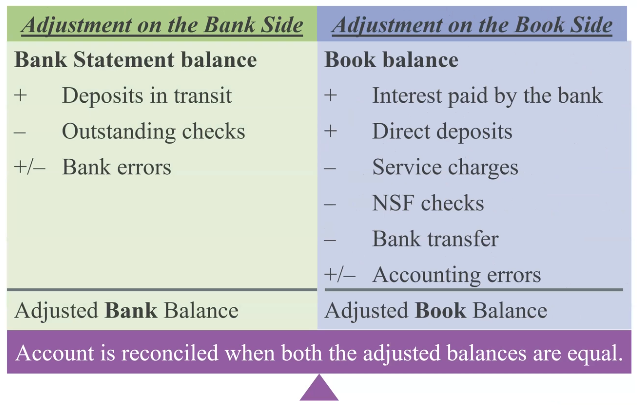
\includegraphics[width=\columnwidth]{image/bank_reconciliation.png}
\end{figure}
\subsubsection{Adjusting entries for the Books}
\begin{itemize}
	\item \textbf{Collection Expense}: expense due to bank
	\item \textbf{Interest Revenue}
	\item \textbf{Miscellaneous Expense}: Bank expenses
	\item To reverse NSF: same as reversing Cash to Accounts Receivable
\end{itemize}
\section{Receivables}
\subsection{Accounts Receivable}
\begin{description}
	\item[Subsidiary accounts] Individual accounts of customers under accounts receivable\\
	e.g. \textit{Accounts Receivable - Customer Name}
	\item[Expected Credit Loss] Alternative names:
	\begin{itemize}
		\item Bad Debt Expense
		\item Accounts Receivable Impairment Loss
		\item Uncollectible Account Expense
	\end{itemize}
    \item[Allowance for Bad Debts/Loss Allowance] a Contra-asset (XA)\\
    Allowance method is preferred under Accrual Accounting Principle as it accounts receivable can be paid by customers in 5 years? 10 years? which might be uncertain
    $$\text{AR} - \text{Loss Allowance} = \text{Net AR}$$
\end{description}
\textbf{How to estimate ending balance for Loss Allowance?}
\begin{itemize}
	\item Individual assessment $\rightarrow$ for customers with known credit problems
	\item Group assessment (\textit{Provision matrix})
	\begin{itemize}
		\item \textbf{Provision matrix}
		\item Aging accounts receivable $\rightarrow$ accounts who have not been paid for longer should have higher probability of not being paid
	\end{itemize}
    \item Result is the ending balance of Loss Allowance Account
\end{itemize}
\subsection{Notes Receivable}
\begin{itemize}
	\item \textbf{Maturity date}: due date; when it is expressed in terms of month, will include the date of issuance, but when expressed in terms of day, will not include the date of issuance but start counting for the day after
	\item \textbf{Interest Revenue}
	$$\text{Interest Revenue} = \text{Face value} \times \text{Annual I/R} \times \text{time period (term)}$$
	\item To record customers who want to pay by notes, we record Dr. Notes Receivable and Cr. Accounts Receivable
	\item When customer makes payment: Dr. Cash and Cr. Notes Receivable + Interest Revenue
	\item To record \textbf{dishonored note receivable}: Dr. Accounts Receivable and Cr. Notes Receivable + Interest Revenue
	\begin{itemize}
		\item Overall effect is an increase in Revenue by the amount equal to Interest Revenue
	\end{itemize}
\end{itemize}
\subsection{Foreign Currency Transaction}
Might happen if transaction is conducted in different currencies (exchange rates fluctuate daily)\\
\textbf{Foreign exchange loss/gain}: A revenue/expense account that is adjusted according to exchange rates\\
\textbf{How to avoid this?}
\begin{itemize}
	\item Denominate price in own currency (US Dollars) and the risk of exchange rate changes would have fallen on the Korean Company
	\item Locked in the price of foreign currency by entering into a forward contract with a foreign currency broker (Derivative contract)
\end{itemize}
\subsection{Variable Consideration}
\textbf{Some examples}
\begin{itemize}
	\item Discounted price for all goods bought if the customer buys a specified quantity
	\item Return policy, but we do not know if the customer will return or not
\end{itemize}
Hence, it is estimated at the start and \underline{is periodically reassessed} using expected value/most likely amount for estimation
\begin{itemize}
	\item Use most likely amount if the outcome is yes/no
	\item Use estimation if there are different outcomes with probabilities
\end{itemize}
\section{Liabilities}
Some recap:
\begin{itemize}
	\item \textbf{Currency}:
	\begin{itemize}
		\item Current if < 1 yr
		\item Non-current if > 1 yr
	\end{itemize}
    \item \textbf{3 Major Uncertainties in Liabilities}
    \begin{itemize}
    	\item Whom to pay
    	\item When to pay
    	\item How much to pay
    \end{itemize}
    \item \textbf{Types of Liabilities}
    \begin{itemize}
    	\item \underline{Known Liabilities}: little uncertainty, who, when and how much is determinable
    	\item \underline{Estimated Liabilities}: a known obligation of an uncertain amount, but one that can be reliably estimated
    	\item \underline{Contingent Liabilities:} potential obligation created as a result of a past event, but which is not yet an effective liability until some future event happens
    \end{itemize}
\end{itemize}
\subsection{Current Liabilities}
\textbf{Current Liabilities}:
\begin{itemize}
	\item GST Payable
	\item Payroll Liabilities: CPF\\
	Employers incur expenses and liabilities from having employees (payroll expenses)
	\begin{itemize}
		\item \textbf{20\% contribution by employee}\vspace{0.5em}\\
		\begin{tabular}{llll}
			\multicolumn{2}{l}{Salaries Expense}& \multicolumn{2}{l}{$x$} \\
			& Salaries Payable - to employee& &80\%$x$\\
			&\multicolumn{3}{l}{CPF Payable - employee contribution}\\
		\end{tabular}\vspace{0.5em}
		\item \textbf{17\% contribution by employer}\vspace{0.5em}\\
		\begin{tabular}{llll}
			\multicolumn{2}{l}{Payroll Expense - CPF}& \multicolumn{2}{l}{$17\%x$} \\
			& CPF Payable - employer contribution& &17\%$x$
		\end{tabular}\vspace{0.5em}
	\end{itemize}
    \item Unearned Revenues
    \item Short-Term (ST) Notes Payable\\
    \impt use 360 days for daily I/R
    \begin{itemize}
    	\item \underline{Entry to record}:
    	\vspace{0.5em}\\
    	\begin{tabular}{llll}
    		\multicolumn{4}{l}{Cash}\\
    		& Notes Payable - Company Name& &
    	\end{tabular}\vspace{0.5em}
    \item \underline{When note is repaid + interest}:\vspace{0.5em}\\
    \begin{tabular}{llll}
    	\multicolumn{4}{l}{Notes Payable - Company Name}\\
    	\multicolumn{4}{l}{Interest Expense (i/r\% $\times$ amt $\times$ days/360)}\\
    	& Cash& &
    \end{tabular}\vspace{0.5em}
\item \underline{End-of-period Adjustments}: Not payable untul the following accounting period, so need to adjust entry at year-end to record the accrued interest expense\vspace{0.5em}\\
\begin{tabular}{llll}
	\multicolumn{4}{l}{Interest Expense (i/r\% $\times$ amt $\times$ days/360)}\\
	& Interest Payable& &
\end{tabular}\vspace{0.5em}
    \end{itemize}
\item \underline{Estimated liabilities}: a known obligation of an uncertain amount, but can be \textbf{reliably estimated}
\begin{itemize}
	\item Warranty Liabilities: to comply with \textbf{full disclosure} and \textbf{matching principles}, the seller reports \textbf{Expected warranty expense} in the period when revenue from the sale is reported\\
	\underline{To record warranty:}\vspace{0.5em}\\
	\begin{tabular}{llll}
		\multicolumn{4}{l}{Warranty Expense ($x\% \times $Sales)}\\
		& Warranty Provision& &
	\end{tabular}\vspace{0.5em}\\
\underline{To record returned items:}\vspace{0.5em}\\
\begin{tabular}{llll}
	\multicolumn{4}{l}{Warranty Provision}\\
	& Inventory& &
\end{tabular}\vspace{0.5em}
\end{itemize}
\item \underline{Contingent liabilities}: potential liabilities that are created as a result of a past event. It is not an effective liability until some future event happens (\eg lawsuits and litigation/legal claims, debt guarantees)

\centering
\begin{tabular}{c|c|c|c}
& probable & \makecell[c]{reasonably\\possible} & remote \\
\hline
estimable & \makecell[c]{\textbf{record as}\\\textbf{liability}} & \makecell[c]{disclose\\in notes} & \makecell[c]{No disclosure\\needed}\\
\hline
\makecell[c]{non-\\estimable} & \makecell[c]{disclose\\in notes} & \makecell[c]{disclose\\in notes} & \makecell[c]{No disclosure\\needed}\\
\end{tabular}\vspace{0.5em}
\begin{itemize}
	\item \textbf{Probable}: chance that the future event/events will occur is high (>50\% for IFRS, >70\% for GAAP)
	\item \textbf{Reasonably possible}: more than remote but less than likely
	\item \textbf{Remote}: chance of occurring is slight
\end{itemize}
\end{itemize}


\section{Inventory}
\textbf{Definition}: Merchandise inventory includes all goods that a company owns and holds for sale, regardless of where the goods are located when inventory is counted
\begin{itemize}
	\item \underline{Goods in Transit}:
	\begin{itemize}
		\item FOB Shipping Point: goods change ownership at shipping point (goods in transit reported as part of buyer's inventory)
		\item FOB Destination
	\end{itemize}
    \item \underline{Goods on Consignment}:
    \begin{itemize}
    	\item Goods the seller (\textbf{consignor}) owns but are on display for sale at another place of business (\textbf{consignee})
    \end{itemize}
\end{itemize}

\subsection{Costs of Inventory}
Cost includes \textbf{all expenditures necessary} to bring an item to a sellable \textbf{condition} and \textbf{location}
\begin{itemize}
	\item Invoice cost
	\item Freight/transport cost
	\item Insurance cost
	\item Storage cost
	\item Import taxes
	\item Less any purchase discounts/returns
\end{itemize}
Note that costs incurred after inventory is ready for use is not included (\eg marketing, salesperson salaries, financing cost, \textbf{Warehouse costs}, \textbf{retail store costs})

\subsection{Perpetual vs Periodic}
\textbf{Perpetual characteristics}:
\begin{itemize}
	\item Up-to-date record maintained
	\item purchases/returns/discounts are directly added to Inventory account
	\item Transaction-by-transaction records
	\item Information on COGS and ending inventory is available on a continuous basis
\end{itemize}
\textbf{Periodic characteristics}:
\begin{itemize}
	\item No p-to-date records during accounting period
	\item purchases/returns/discounts are recorded in a temporary account (\textbf{NOT} Inventory)
	\item Actual physical count of inventory is done at the end of the period
	\item COGS is then calculated indirectly using the COGS equation
\end{itemize}

\subsubsection{Periodic Inventory}
$$\text{Beg. Inventory} + \text{Net Purchases} = \text{COGS} + \text{End Inventory}$$
\textbf{Types of temporary accounts}:
\begin{itemize}
	\item Purchases
	\item Freight-in: to take into account transport costs, because COGS is unknown
	\item Purchase returns
	\item Purchase discounts: might happen when the company pays invoice before the due date and gets discount
\end{itemize}
\textbf{Steps to take at the end of the period}:
\begin{itemize}
	\item Temporary accounts will all be closed to the inventory account at the end of the period
	\item COGS will be computed after physical count and using other COGS method, and debit COGS and credit Inventory
\end{itemize}

\subsubsection{Perpetual Inventory}
What happens if there's inventory shrinkage (\textbf{loss of merchandise})?
\begin{itemize}
	\item Debit COGS and Credit Inventory (since we don't know what happens to the lost goods, we just assume that they're sold)
\end{itemize}
\textbf{Advantage of perpetual system}:
\begin{itemize}
	\item up-to-date count helps to confirm the amount in the accounting system or highlight shortages of inventory
\end{itemize}

\subsection{Inventory Costing Methods}

\subsubsection{Specific Identification Method}
\begin{itemize}
	\item When specific units are sold, the specific cost of that unit is recorded as COGS.
	\item Impractical for large quantities of similar items being sold (e.g. toothpaste, clothing etc…)
	\item Typically used when dealing with expensive unique items (e.g. houses, expensive fine jewelry, unique custom made cars etc…) where costs can be easily tracked to specific item
\end{itemize}
\subsubsection{FIFO}
\textbf{Advantage}:
\begin{itemize}
	\item Ending inventory approximates current replacement cost
\end{itemize}
\subsubsection{LIFO}
\textbf{Advantage}:
\begin{itemize}
	\item Better matches current costs in COGS with revenues
\end{itemize}
\subsubsection{Average Cost Method}
\begin{itemize}
	\item When a unit is sold, the avg cost per unit is assigned to COGS
	$$\text{Avg Cost} = \frac{\text{Cost of Goods available for Sale}}{\text{Number of units available for sale}}$$
\end{itemize}
\textbf{Advantage}:
\begin{itemize}
	\item Smooth out price changes
\end{itemize}
\subsection{Net Realizable Value (NRV)}
\begin{itemize}
	\item Ending inventory has to be reported at the \textbf{lower of cost or market value}
	\item Meaning that if the replacement cost of the same goods in inventory is lower than the inventory cost, it has to report the market value instead.
	\item NRV can be applied in two ways:
	\begin{itemize}
		\item Separately to each individual item
		\item To major categories of assets
	\end{itemize}
\end{itemize}
\textbf{What happens if NRV < Initial cost}? Need to make a journal entry to change Net Inventory\vspace{0.5em}\\
\begin{tabular}{llll}
	\multicolumn{4}{l}{Cost of Goods Sold}\\
	& Allowance for Inventory Write Down& &
\end{tabular}\vspace{0.5em}\\
Where the above is a \textbf{XA} account to Inventory
$$\text{Net Inventory} = \text{Inventory} - \text{Less: Allowance for Write-Down}$$

\section{PPE}
\textbf{Types of Assets}:
\begin{itemize}
	\item Tangible: \underline{PPE} (Fixed assets such as land, building, equipment) + \underline{Natural resources} (mineral deposits, oil fields)
	\item Intangible:
	\begin{itemize}
		\item \underline{Definite life}: patents, copyright, franchises, licenses
		\item \underline{Indefinite life}: trademarks, goodwill
	\end{itemize}
\end{itemize}
\subsection{Acquiring PPE}
PPE (tangible assets actively used in operations that will give future benefits) are initially recorded at \textbf{COST} \impt
\begin{itemize}
	\item Including the purchase price and all \underline{expenditures needed to prepare the asset} for its intended use.
	\begin{figure}[H]
		\centering
		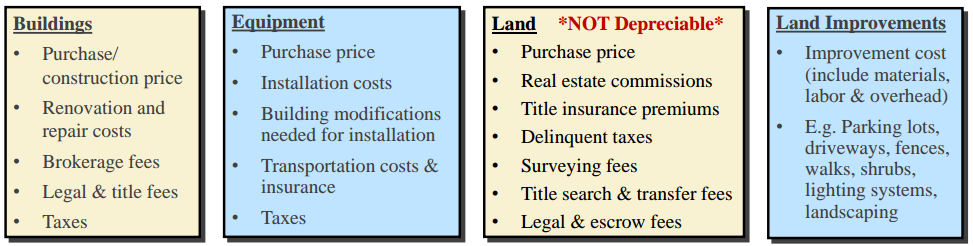
\includegraphics[width=\columnwidth]{image/ppe_acquisition}
	\end{figure}
    \item \textbf{Lump-sum purchase}: buying different assets at a combined cost, usually in total smaller than buying individual assets
    \begin{itemize}
    	\item total cost of a combined purchase is \underline{separated} on the basis of the \textbf{relative fair market values} of each asset component
    \end{itemize}
\end{itemize}
\subsection{Depreciation}
\begin{itemize}
	\item Use Depreciation Expense and Accumulated Depreciation (XA) Accounts
	\item \textbf{Net Book Value} (\textbf{carrying amount}) is the 'current' value of the asset
	$$\text{NBV} = \text{Acquisition Cost} - \text{Accumulated Depreciation}$$
\end{itemize}
\textbf{Some depreciation methods}: to calculate Depreciation Expense
\begin{itemize}
	\item \underline{Straight-line method}
	\item \underline{Unit-of-production method} (used for depletion of natural resources also, but this one need to estimate the usable value of all the natural resources)
	\item \underline{Double-Declining Balance (DDB)}: usually use multiplier=2
	$$\text{Depreciation Expense} = \text{Current NBV} \times \frac{\text{Multiplier}}{\text{Useful life in yrs}}$$
\end{itemize}
\impt \textbf{Partial-Year Depreciation}: Note that if we buy an equipment in the middle of the year, the depreciation expense for the year is only \underline{a proportion} of annual depreciation expense
\begin{itemize}
	\item in the last year, the depreciation would be also a portion of the annual dep. expense since the PPE is supposed to end its life in the middle of the year
\end{itemize}
\textbf{Changes in Depreciation estimate}:
\begin{itemize}
	\item Need to estimate \textbf{Residual Value} and \textbf{Useful Life}, but this may change
	\item \impt If it changes, it does not affect past years' depreciation expense, only affects future years!
\end{itemize}
\subsection{Capitalize or Expense?}
\begin{itemize}
	\item \textbf{R\&D}: Research cost are expensed. Development cost after technological feasibility is established can be capitalized. (IFRS)
	\item \textbf{PPE:} If we capitalize, there would be less expense and this would boost income (WorldCom scandal where revenues were boosted and assets were inflated)
	\begin{figure}[H]
		\centering
		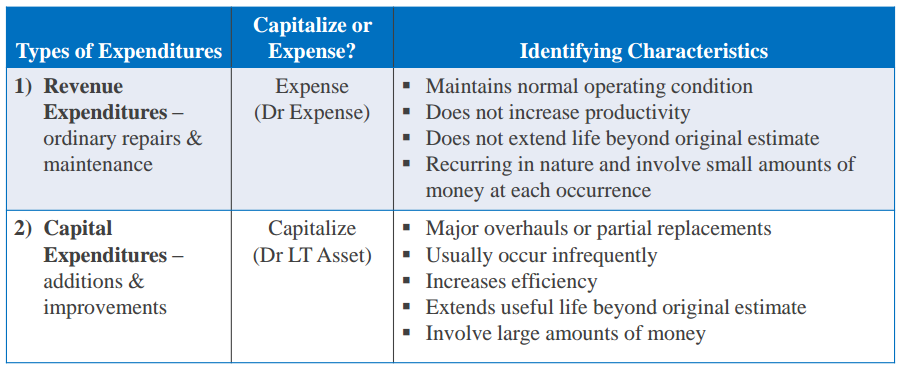
\includegraphics[width=\columnwidth]{image/cap_exp.png}
	\end{figure}
\end{itemize}
\subsection{Impairment of PPE}
\textbf{Definition}:An impairment is the amount by which the \textbf{carrying amount} of an asset exceeds its \textbf{recoverable amount}.
\begin{itemize}
	\item Journal entry:\vspace{0.5em}\\
	\begin{tabular}{llll}
		\multicolumn{4}{l}{Impairment loss on Equipment}\\
		& Accumulated Impairment Loss& &
	\end{tabular}\vspace{0.5em}\\
    \item Impairment loss: classified under equity and included under IS
    \item Accumulated Impairment Loss: classified under XA
\end{itemize}
\subsection{Disposal of PPE}
\textbf{Steps to record Disposal}
\begin{itemize}
	\item Need to update depreciation expense and add to the accumulated depreciation account first
	\item Journal entry if there is gain from selling\vspace{0.5em}\\
	\begin{tabular}{llll}
		\multicolumn{4}{l}{Cash}\\
		\multicolumn{4}{l}{Accumulated Depreciation}\\
		& PPE& &\\
		& Gain on Sale of Asset
	\end{tabular}
    \item Note that Disposal is usually classified under \underline{Accumulated Depreciation and Impairment}
    \item Note that Gain on Disposal is usually classified under \underline{Operating Profit}
\end{itemize}
\subsection{Intangible Assets}
\textbf{Types}:
\begin{itemize}
	\item \textbf{Definite Life}: Amortise over its estimated useful life. Usually assumed to have 0 salvage value (use straight-line method, similar to depreciation but use \textbf{Amortisation expense} and \textbf{Accumulated Amortisation})
	\begin{itemize}
		\item \textbf{Patents}: granted by the government for an invention, exclusive right for owner to use, manufacture and sell the product of the patent
		\item \textbf{Copyrights}: exclusive rights to publish, use and sell literary, musical or artistic work.
		\item \textbf{Franchises}: contractual right to sell certain products or services, use certain trademarks, or perform activities in a certain region
	\end{itemize}
    \item \textbf{Indefinite Life}: Not amortised, but tested at least annually for possible impairment, and book value is reduced to fair value if impaired.
    \begin{itemize}
    	\item \textbf{Trademarks}: exclusive legal right to use a distinctive name, image or slogan.
    	\item \textbf{Goodwill}: when one company buys another company, the \textit{excess} of the purchase price over the fair market value of acquired net assets is goodwill. (Note that only \underline{purchased} goodwill is an intangible asset!)
    \end{itemize}
\end{itemize}
\impt “Intangibles” that are NOT acquired through an exchange is NOT recorded in the company’s books!

\section{Equity}
\textbf{Capital Structure!}: Debt vs Equity
\begin{itemize}
	\item How much of the company's funds are coming from debts vs equity
	\item Loans (\underline{Debt Financing}): Company is obligated to repay the principal amount
	\item Investment (\underline{Equity Financing}): Company is not obligated to repay the principal amount
\end{itemize}
\subsection{Ownership of a corporation}
\textbf{Rights as shareholders/stockholders}:
\begin{itemize}
	\item Vote at shareholders' meetings
	\item Purchase additional shares/ sell shares
	\item Receive dividends (dividends rights): proportionate share on the distribution of profits
	\item Residual claims
	\begin{itemize}
		\item Can get proportionate share on the distributions of remaining assets upon liquidation of the company
		\item Note that creditors are paid before shareholders in the event of liquidation or bankruptcy\vspace{0.5em}
	\end{itemize}
\end{itemize}
\textbf{Composition of a company's shares}
$$\text{Authorized Shares} = \text{Outstanding} + \text{Treasury} + \text{Unissued}$$
\begin{itemize}
	\item Authorized = max number of shares that can be sold to the public (stated in corporate charter)
	\item Outstanding = issued shares that are owned by stockholders
	\item Treasury = issued shares that have been reacquired by the corporation
	\item Issued = authorized shares of stocks that have been sold (Outstanding + Treasury)
	\item Unissued = authorized shares that have never been sold
\end{itemize}
\textbf{What is par value?}
\begin{itemize}
	\item Par-value: is an arbitrary amount assigned to each stock when it is authorized
	\item \textbf{Premium}: When par-value stock sells for above par
	\item No-par-value: no arbitrary amount is assigned (SG uses no par value)
\end{itemize}
\textbf{IPO\& SEO}
\begin{enumerate}
	\item \textbf{Initial Public Offering (IPO)}: the first time a corporation sells share to the public
	\item \textbf{Secondary/Seasoned Equity Offering (SEO)}: subsequent sales of new shares to the public
	\item Once the initial sale of shares is done, investors can sell their shares to other investors in secondary markets (NYSE, SGX, HKSE)
\end{enumerate}


\subsubsection{Ordinary shares}
\textbf{Par value shares}
\begin{itemize}
	\item \underline{Issuance for cash at premium} \vspace{0.5em}\\
	\begin{tabular}{llll}
		\multicolumn{4}{l}{Cash (amt $\times$ mkt value)}\\
		& Common Stock (amt $\times$ par value)& &\\
		& Paid-in capital in excess of par& &
	\end{tabular}\vspace{0.5em}\\
\item \underline{Issuance for acquisition of asset}: based on market value of shares if the mkt value of the asset cannot be determined \vspace{0.5em}\\
\begin{tabular}{llll}
	\multicolumn{4}{l}{Land (amt $\times$ mkt value)}\\
	& Common Stock (amt $\times$ par value)& &\\
	& Paid-in capital in excess of par& &
\end{tabular}\vspace{0.5em}\\
\end{itemize}
\textbf{No par shares}
\begin{itemize}
	\item \underline{Issuance for cash} \vspace{0.5em}\\
	\begin{tabular}{llll}
		\multicolumn{4}{l}{Cash }\\
		& Common Stock (ordinary no par shares)& &
	\end{tabular}\vspace{0.5em}\\
	\item \underline{Issuance for acquisition of asset}: based on market value of asset \vspace{0.5em}\\
	\begin{tabular}{llll}
		\multicolumn{4}{l}{Equipment}\\
		& Common Stock (ordinary no par shares)& &
	\end{tabular}\vspace{0.5em}\\
\item \underline{Issuance of stated value shares}: if market value > stated value, premium = market value - stated value \vspace{0.5em}\\
\begin{tabular}{llll}
	\multicolumn{4}{l}{Cash}\\
	& Common Stock - ordinary no par shares& &\\
	& Common Stock Premium - ordinary
\end{tabular}
\end{itemize}

\subsubsection{Preferred Shares}
\textbf{Reasons for issuing preference shares:}
\begin{itemize}
	\item Raise capital without sacrificing control
	\item Boost the return earned by ordinary shareholders through \underline{financial leverage}
	\item To appeal to investors who may believe the ordinary shares are too \underline{risky} or that the expected return on ordinary shares is too low
\end{itemize}
\textbf{Types of preferred shares}:
\begin{itemize}
	\item Convertible: can be converted to ordinary shares
	\item Redeemable: company can buy back the shares
	\item Cumulative: require all dividends in arrears (outstanding unpaid dividends from past years) to be fully paid before ordinary dividends can be paid out
	\item Participating: receive additional dividend based on predetermined condition
\end{itemize}
\textbf{Issuance of no par preferred shares:}\vspace{0.5em}\\
\begin{tabular}{llll}
	\multicolumn{4}{l}{Cash}\\
	& Preferred Stock - Class E& &\\
\end{tabular}\vspace{0.5em}\\
\textbf{Issuance of par value preferred shares:}\vspace{0.5em}\\
\begin{tabular}{llll}
	\multicolumn{4}{l}{Cash}\\
	& Preferred Stock - Class E& &\\
	& Paid-in Capital in Excess of par, preferred
\end{tabular}\vspace{0.5em}\\

\subsubsection{Treasury Shares}
\textbf{Reasons companies may want to buy back its shares from existing shareholders}
\begin{itemize}
	\item Use their shares to acquire other companies
	\item Avoid a hostile takeover
	\item Reissue to employees as compensation
	\item Show management's confidence in the current price (stimulate trading??)
	\item Give cash back to shareholders?
	\item Increase reported earnings per share (EPS) by reducing number of shares outstanding (refer to FSA)
\end{itemize}
\impt Note that treasury shares is recorded at cost, and it is a \textbf{Contra-Equity Account}
\begin{tabular}{llll}
	\multicolumn{4}{l}{Treasury Shares}\\
	& Equity& &\\
\end{tabular}\vspace{0.5em}\\
Reissuance of Treasury Shares
\begin{itemize}
	\item \underline{At cost}\vspace{0.5em}\\
	\begin{tabular}{llll}
		\multicolumn{4}{l}{Cash}\\
		& Treasury Shares& &\\
	\end{tabular}\vspace{0.5em}\\
	\item \underline{Higher than cost}\vspace{0.5em}\\
	\begin{tabular}{llll}
		\multicolumn{4}{l}{Cash}\\
		& Treasury Shares& &\\
		& Premium on Treasury shares & &
	\end{tabular}\vspace{0.5em}\\
	\item \underline{Lower than cost} (sufficient balance in 'Treasury share premium' account): need to deduct premium account \vspace{0.5em}\\
	\begin{tabular}{llll}
		\multicolumn{4}{l}{Cash}\\
		\multicolumn{4}{l}{Premium on treasury shares}\\
		& Treasury shares & &
	\end{tabular}\vspace{0.5em}\\
	\item \underline{Lower than cost} (insufficient balance in 'Treasury share premium' account): will need to deduct RE and premium accounts\vspace{0.5em}\\
	\begin{tabular}{llll}
		\multicolumn{4}{l}{Cash}\\
		\multicolumn{4}{l}{Premium on treasury shares}\\
		\multicolumn{4}{l}{Retained Earnings}\\
		& Treasury shares& &
	\end{tabular}\vspace{0.5em}\\
\end{itemize}

\subsection{Dividends}
\begin{itemize}
	\item \textbf{Types of dividends}: Cash and Stock
	\item \textbf{Requirements to declare and pay dividends}
	\begin{itemize}
		\item Sufficient balance in RE
		\item Sufficient cash to pay for cash dividends
	\end{itemize}
\end{itemize}
\subsubsection{Cash Dividends}
\underline{Three important dates}
\begin{itemize}
	\item \textbf{Declaration date}: board declares the dividends, company records a liability\vspace{0.5em}\\
	\begin{tabular}{llll}
		\multicolumn{4}{l}{Dividends - Ordinary Shares}\\
		& Dividends Payables & &
	\end{tabular}\vspace{0.5em}\\
\item \textbf{Date of record}: Stockholders holding shares on this date will receive the dividend
\item \textbf{Payment date}: Company pays the dividends\vspace{0.5em}\\
\begin{tabular}{llll}
	\multicolumn{4}{l}{Dividends Payables}\\
	& Cash & &
\end{tabular}\vspace{0.5em}\\
\end{itemize}
\impt Note that Dividends are temporary accounts so need to be closed at the end of FY to RE\vspace{0.5em}\\
\textbf{Distribution of preferred dividends}
\begin{itemize}
	\item \textbf{Current-Dividend Preference}
	\begin{itemize}
		\item Preferred are prioritized first before common receive dividends
	\end{itemize}
    \item \textbf{Cumulative-Dividend Preference}
    \begin{itemize}
    	\item Preferred stockholders paid \underline{dividends in arrears} and current dividends before common stockholders receive any if at all
    	\item \textbf{Dividends in arrears}: unpaid dividends from past years
    	\item Dividends in arrears do not represent actual liabilities, so not recorded in accounts, but is \textit{recorded in notes to FS}
    \end{itemize}
\end{itemize}

\subsubsection{Stock Dividends}
\textbf{Definition}: issue new shares to its shareholders without receiving cash (There is no total change in Equity since Dividends is closed to RE at the end of FY)
\begin{itemize}
	\item Small dividends (<20-25\% of issued shares): assign \underline{fair value} because at the end of FY it won't affect RE much
	\item Large dividends (>25\% of issued shares): assign \underline{par value} because if fair value was used it would increase RE greatly
\end{itemize}
\underline{Issuance of small stock dividends}: fair value
\begin{itemize}
	\item \textbf{Declaration date}:\vspace{0.5em}\\
	\begin{tabular}{llll}
		\multicolumn{4}{l}{Stock Dividends (amt $\times$ fair value)}\\
		& Stock Dividends Distributable & &\\
		& Paid-in Capital in Excess of Par& &
	\end{tabular}\vspace{0.5em}\\

	\item \textbf{Distribution date}:\vspace{0.5em}\\
	\begin{tabular}{llll}
		\multicolumn{4}{l}{Stock Dividends Distributable}\\
		& Common Stock& &
	\end{tabular}\vspace{0.5em}\\
\item \textbf{Closing at the end of FY}: Move everything to RE
\end{itemize}
\underline{Issuance of large stock dividends}: par value
\begin{itemize}
	\item \textbf{Declaration date}:\vspace{0.5em}\\
	\begin{tabular}{llll}
		\multicolumn{4}{l}{Stock Dividends (amt $\times$ par value)}\\
		& Stock Dividends Distributable & &\\
	\end{tabular}\vspace{0.5em}\\

	\item \textbf{Distribution date}:\vspace{0.5em}\\
	\begin{tabular}{llll}
		\multicolumn{4}{l}{Stock Dividends Distributable}\\
		& Common Stock& &
	\end{tabular}\vspace{0.5em}\\
	\item \textbf{Closing at the end of FY}: Move everything to RE
\end{itemize}
\impt \textbf{Stock Split}: increasing number of shares outstanding in the same proportion that par or stated value per share decreases such that equity remains unchanged\\
\impt Both Stock Split and Stock Dividends will increase total shares outstanding $\Rightarrow$ will decrease market value/price

\section{Statement of Cash Flow (SCF)}
\textbf{Importance of positive cash flow?}
\begin{itemize}
	\item Drives daily operations
	\item Increases purchasing power
	\item Allows for expansion and new investment opportunities
	\item Greater protection against creditors
	\item Gives greater flexibility to respond to critical situations (protection in the future)
	\item Allows company to pay dividends to owners
\end{itemize}
\textbf{Cash includes}:
\begin{itemize}
	\item Currency
	\item Cash equivalents: \underline{short-term highly liquid} investments that are readily converted into cash, usually with extremely \underline{short maturity dates} (less than 3 months) such that there's little to no risk of value changing due to i/r changes
\end{itemize}
\textbf{Classification of activities}
\begin{itemize}
	\item \textbf{Operating}: related to earnings from \underline{normal operations} (the principal revenue-producing activities)
	\begin{itemize}
		\item Customers
		\item Royalties, fees, commision, other revenue
		\item Purchase of goods and services from suppliers
		\item Salaries and wages
		\item Income taxes
		\item Other operating expenses (rent, utilities)
	\end{itemize}
	\item \textbf{Investing}: related to the \underline{acquisition} and \underline{disposal} of long-term assets and other investments
	\begin{itemize}
		\item Purchase/Sale/Disposal of PPE \& other Long-term Assets
		\item Purchase/Sale or maturity or investments in securities
		\item Cash received from repayment of loans made to other parties
		\item Cash paid for loans made to other parties
	\end{itemize}
	\item \textbf{Financing}: related to external sources of \underline{financing} (owners and creditors)
	\begin{itemize}
		\item Cash received from borrowings on loans, notes, bonds
		\item Cash received from issuing shares to owners
		\item Cash paid for repayment of principal to creditors
		\item Cash paid for repurchasing shares to shareholders
		\item Dividends to owners
	\end{itemize}
\end{itemize}
\begin{figure}[H]
	\centering
	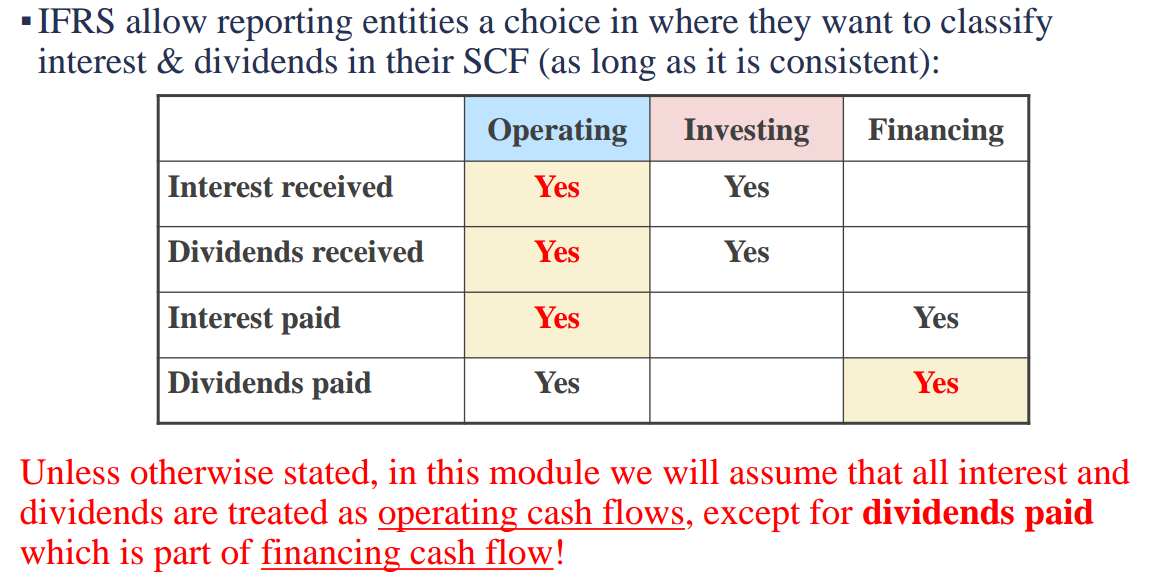
\includegraphics[width=\columnwidth]{image/intdiv.png}
\end{figure}
\textbf{Information needed to prepare SCF}:
\begin{enumerate}
	\item Comparative Balance Sheets/SFPs
	\item Current IS
	\item Additional Details concerning selected accounts
\end{enumerate}
\subsection{Cash Flows from Operating Activities (CFO)}
%%%%% why



\textbf{Two Methods}:
\begin{itemize}
	\item \textbf{Indirect method}: start with accrual profit before tax and deduct/add components if they overstate/understate cash flows
	$$\text{Net Income} +/- \text{Adjustments} = \text{CFO Cash Flow}$$
	Note that this is possible because
	\begin{equation*}
		\begin{aligned}
\text{Assets} &= \text{Liabilities} + \text{Equity}\\
\text{Cash}  &= \text{Liabilities} + \text{Equity} - \text{Non-Cash Assets}\\
\Delta\text{Cash} &= \Delta\text{Liabilities} + \Delta\text{Equity} - \Delta\text{Non-cash assets}
		\end{aligned}
	\end{equation*}
\begin{figure}[H]
	\centering
	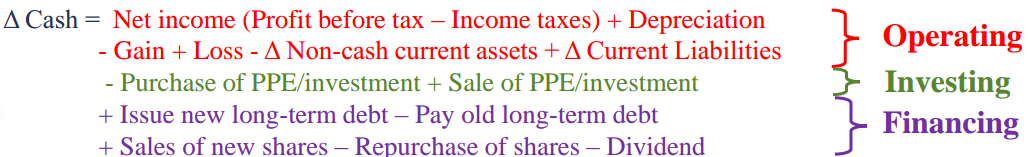
\includegraphics[width=\columnwidth]{image/magic.png}
\end{figure}
	\item \textbf{Direct method}: rarely used,
	$$\text{Cash Sales} - \text{Cash Expenses} = \text{CFO Cash Flows}$$
\end{itemize}
\subsubsection{Indirect Approach}
\begin{enumerate}
	\item Start with \textbf{Profit Before Tax}
	\item + Depreciation/Amortization expenses
	\begin{itemize}
		\item No cash involved in these expenses, so we add it back
	\end{itemize}
    \item Decrease (Increase) in Non-cash Current Assets
    \item Increase (Decrease) in Current Liabilities
    \item -Gain / +Loss on disposal of long-term assets
    \begin{itemize}
    	\item This is reported under the CFI (Investing Activities) section and so is a non-operating activity, so we have to adjust them to avoid \underline{double counting}
    \end{itemize}
    \item +Interest Expense
	\item -Interest Income
	\item -Dividend Income
    \item \textbf{Calculate} \underline{Cash generated from operations}
    \item +Interest Income received
    \begin{itemize}
    	\item actually received in cash (after taking into account receivables)
    \end{itemize}
    \item -Income taxes paid
    \begin{itemize}
    	\item actually paid in cash (after taking into account payables)
    \end{itemize}
    \item \textbf{Calculate} \underline{Net cash from operating activities}
\end{enumerate}

\subsubsection{How to analyze CFO}
CFO measures firm's ability to \underline{generate cash internally} through operations and its management of current assets and current liabilities
\begin{itemize}
	\item \textbf{Investors} will not invest in a company if they do not believe that cash generated from operations will be available to pay them \underline{dividends} or \underline{expand} the company
	\item \textbf{Creditors} will not lend money if they do not believe that cash generated from operations will be available to pay back the loan
	\item Accounts Receivable: Sometimes managers want to boost sales by extending credit terms $\Rightarrow$ $\uparrow$ Accounts Receivable but Cash flow stays approximately constant
	\begin{itemize}
		\item Net Income will outpace cash flows
	\end{itemize}
    \item Inventory changes
    \begin{itemize}
    	\item $\uparrow$Inventory can indicate a planned sales growth that did not materialize
    	\item $\downarrow$Inventory can be a sign that the company is anticipating lower sales in the next quarter
    \end{itemize}
\end{itemize}

\subsection{Cash Flows from Investing Activities (CFI)}
\textbf{Steps}:
\begin{enumerate}
	\item Use Comparative SFP to calculate accounts changes for CFI items in the SFP
	\item Use additional information (\eg purchase/sale of fixed assets, purchase/sale of investments)
\end{enumerate}

\subsection{Cash Flows from Financing Activities (CFF)}
\textbf{Steps}:
\begin{enumerate}
	\item Use Comparative SFP to calculate accounts changes for CFF items in the SFP
	\item Use additional information (\eg sale/repurchase of stock, divident payments, borrowings)
\end{enumerate}
$$\Delta \text{Cash} = \text{CFO + CFI + CFF}$$
$$\text{Ending Cash (SFP)} = \text{Beg. Cash} + \Delta\text{Cash}$$

\section{Ratios}
\textbf{General areas of FSA}:
\begin{itemize}
	\item \textbf{Liquidity and efficiency}: able to meet \underline{short term obligations} and efficiently generate revenues
	\item \textbf{Solvency}: able to meet \underline{long term obligations} and generate \underline{future} revenues
	\item \textbf{Profitability}: rewards for investors
	\item \textbf{Cash Flow}: manage cash inflow and outflow
	\item \textbf{Market Prospects}: generate positive market expectations
\end{itemize}


\subsection{Return on Assets (ROA)}
\begin{equation*}
	\begin{aligned}
		\text{ROA} &= \frac{\text{Net profit}}{\text{Avg total assets}}
		%&= \frac{\text{Net profit}}{\frac{\text{balance_{beginning}} + \text{balance_{ending}}}{2}}
	\end{aligned}
\end{equation*}
Measures \textit{profitability}
\subsection{Debt Ratio}
\begin{equation*}
	\begin{aligned}
		\text{Debt Ratio} = \frac{\text{Total Liabilities}}{\text{Total Assets}}
	\end{aligned}
\end{equation*}
Measures \textit{solvency} and financial leverage (higher financial leverage $\Rightarrow$ higher risk)
\subsection{Profit Margin/Return on Sales}
$$\text{Profit Margin} = \frac{\text{Net Income/Profit}}{\text{Net Sales}}$$
\textit{Profitability?}: How much profit is generated every one dollar of sales?
\begin{itemize}
	\item Measures future growth of the company
	\item Start-ups will usually have negative growth, but if it's decreasing in magnitude it's good
\end{itemize}

\subsection{Accounts Receivable Turnover}
$$\text{Accounts Receivable Turnover} = \frac{\text{Net Sales Revenue}}{\text{Average Accounts Receivable}}$$
Measures how well an organization is managing its accounts receivable (collecting receivables/cash, paying short-term loans to cover cash shortage)
$$\text{Average Collection Period} = \frac{365}{\text{Accounts Receivable Turnover}}$$

\subsection{Current Ratio}
$$\text{Current Ratio} = \frac{\text{Current Assets}}{\text{Current Liabilities}}$$
Measures ability of a company to pay its short-term obligations with short-term assets (\textit{liquidity})\\
\textbf{liquidity}: how easily an asset can be converted to cash\\
But too high ratio can indicate the firm might not be using resources efficiently

\subsection{Acid-Test Ratio (Quick Ratio)}
$$\text{Acid-Test Ratio} = \frac{\text{Quick Assets}}{\text{Current Liabilities}}$$
\begin{equation*}
\begin{aligned}
\text{Quick Assets} = &\text{Cash} + \text{Short-Term Investments}\\
 &+ \text{Current Trade Receivables}
\end{aligned}
\end{equation*}
Measures a company's ability to quickly pay its short-term obligations using liquid assets (exclude inventory, prepaid, and other current assets)\\
Useful to assess if the company will face \textit{near-term liquidity problems}
\begin{itemize}
	\item If Quick Ratio $\geq$ 1.0 then near-term liquidity problems are unlikely, and vice-versa
\end{itemize}

\subsection{Inventory Turnover}
$$\text{Inventory Turnover} = \frac{\text{COGS}}{\text{Average Inventory}}$$
Measures how many times a company turns over (sells) its inventory
Measures liquidity (if the company is controlling inventory well)

$$\text{Days' Sales in Inventory} = \frac{365}{\text{inventory Turnover}}$$
Estimates \textit{how many days on average it will take to convert inventory to cash/AR}

\subsection{Operating Cycle of a Company}
\begin{equation*}
\begin{aligned}
\text{Operating Cycle Length} = & \text{Avg Collection Period} \\&+ \text{Days in Inventory}
\end{aligned}
\end{equation*}
Measures: \textit{how much time it takes} from the point inventory is purchased to cash collection from customer

\subsection{Number of Days' Purchases in Accounts Payable}
$$\text{Days' Purchases in AP} = \frac{365}{\frac{\text{Purchases}}{\text{Avg Accounts Payable}}}$$

Measures how many days' worth of inventory does the company have in accounts payable
\begin{itemize}
	\item Avg. length of time between \textbf{purchases} of inventory (on credit) and \textbf{cash payment for that inventory}
	\item Useful to assess \textbf{how fast} a company is in paying its suppliers
	\begin{figure}[H]
		\centering
		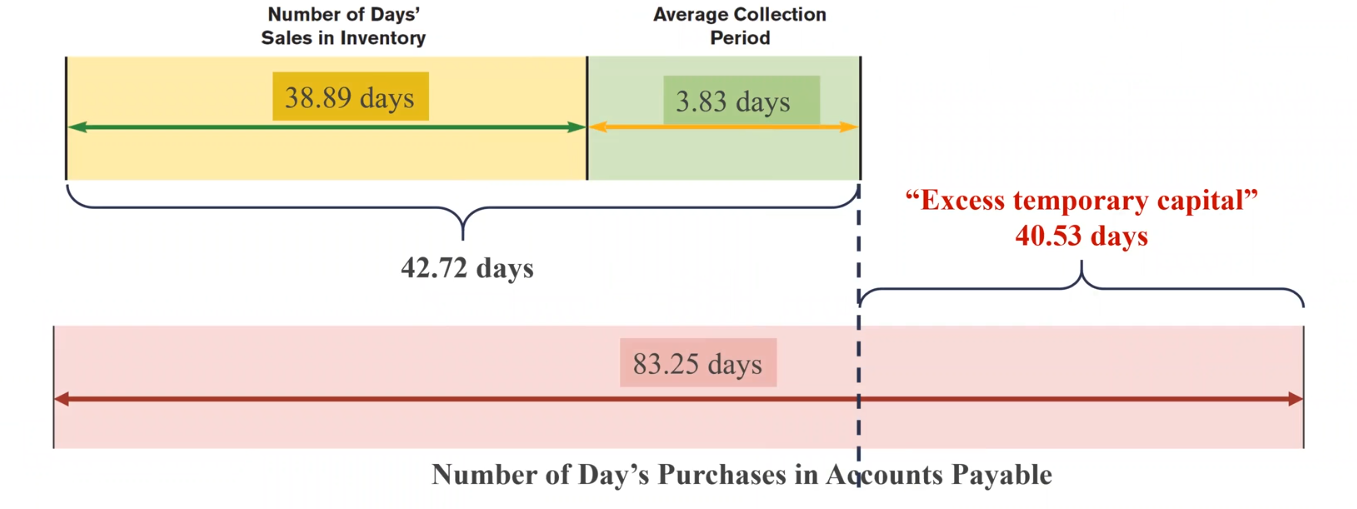
\includegraphics[width=\columnwidth]{image/operating_cycle.png}
		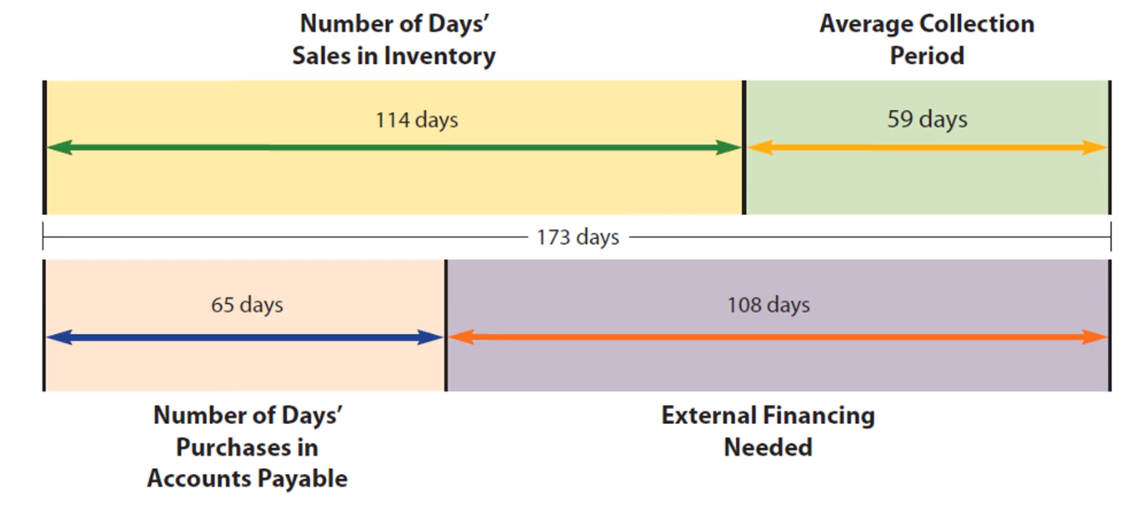
\includegraphics[width=\columnwidth]{image/caterpillar_opcycle.png}
	\end{figure}
    \item Does the company need to rely on \textbf{external financing} for cash to support its operating activities
\end{itemize}

\subsection{Fixed Assets Turnover (PPE Turnover Ratio)}
$$\text{FA Turnover} = \frac{\text{Net Sales}}{\text{Average Fixed Assets}}$$
$$\text{Avg. Fixed Assets} = \text{Avg. PPE}$$
\textit{Measures how efficient a company is in using its fixed assets to generate sales} (\underline{Profitability})
\begin{itemize}
	\item How much sales is generated per each dollar (unit) of PPE?
\end{itemize}

\subsection{Total Assets Turnover}
$$\text{TA Turnover} = \frac{\text{Net Sales}}{\text{Average Assets}}$$
\textit{Measures how efficient a company is in using its assets as a whole to generate sales} (\underline{Profitability})

\subsection{Earnings per Share (EPS)}
$$
\text{EPS} = \frac{\text{Net Profit} - \text{Preferred Dividends}}{\text{Weighted-average Ordinary Shares Outstanding}}
$$
\impt Measures \underline{profitability}: ability to produce income for each ordinary share outstanding
\begin{itemize}
	\item Required to disclose on the IS!
	\item \textbf{Diluted EPS}: EPS but assumes that all convertible securities are converted into ordinary shares
\end{itemize}

\subsection{Price-Earnings (PE) Ratios}
$$
\text{PE Ratio} = \frac{\text{Mkt value (price) per share}}{EPS}
$$
Assessing \textbf{Market expectations}: Measures what the market is willing to pay for the company current earnings stream
\begin{itemize}
	\item High ratio means that a company is overpriced (too high expectations for low earnings)
\end{itemize}

\subsection{Dividend Payout Ratio}
$$\text{Dividend Payout Ratio} = \frac{\text{Cash Dividends}}{\text{Net Income}}$$
Measures the percentage of net income paid out during the year in the form of cash dividends (for Net Income use profit for the year/profit attributable to owners of the company)
\begin{itemize}
	\item \textbf{Income shares}: companies that consistently pay large dividends
	\item \textbf{Growth shares}: companies that distribute little to no dividends, because usually profits are reinvested back to generate bigger revenues for the company
\end{itemize}

\subsection{SCF Analysis}
\begin{figure}[H]
	\centering
	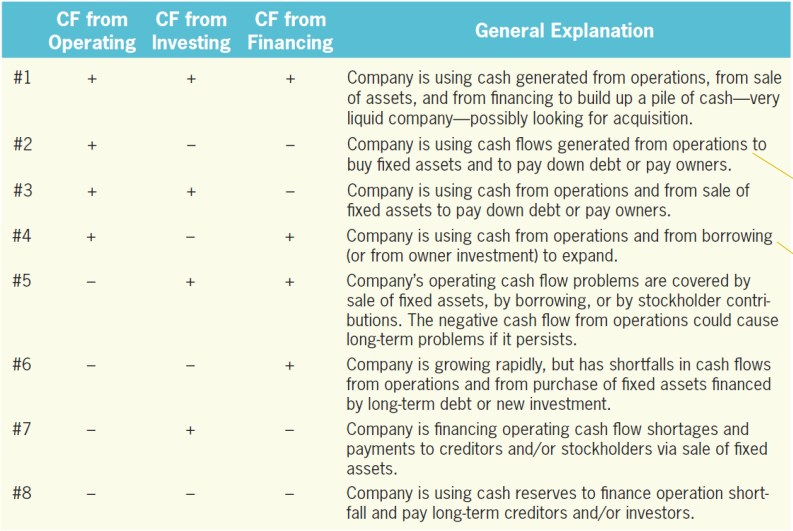
\includegraphics[width=\columnwidth]{image/scf_analysis.png}
\end{figure}

\section{Financial Statement Analysis (FSA)}
\begin{itemize}
	\item Help users make better economic decisions [External parties and Internal (Management)]
	\item Financial
\end{itemize}

\section{Exam stuff}
\begin{itemize}
	\item Record transactions: prepare journal entries
	\item prepare ledger: draw T-accounts
	\item on credit = on account
	\item Property Plant and Equipment: it's very broad and if we want to record in journal entry usually need specific accounts
	\item Write "not included in journal" when there's no exchange of goods/cash
\end{itemize}
\end{multicols}











\end{document}